\section{Background and Main Ideas}

This section describes the key idea of SampleClean, namely, that data cleaning can be integrated with approximate query processing leading to bounded approximations of clean query results for a fraction of the cleaning cost.

\subsection{Data Cleaning is Often Expensive}
A number of surveys report that data cleaning is one of the most time consuming steps \cite{kandel2012enterprise, nytimes}.
Data cleaning frameworks have been recently proposed to address the problem of corrupted data at scale\cite{khayyat2015bigdansing, chu2015katara, sampleclean}.
As errors can be domain- or dataset-specific, data cleaning is an inherently human-driven process and can require a significant amount of developer effort in writing software or rules to fix the corruption.
Automated fixes may not be reliable and can require human confirmation \cite{DBLP:journals/pvldb/YakoutENOI11}.
One way to scale up human computation is crowdsourcing which has shown recent success in entity resolution and value filling \cite{gokhale2014corleone, park2014crowdfill, sampleclean,chu2015katara}.
However, crowdsourcing comes with the costs of significant additional latency (orders of magnitude slower than data processing) and the overhead of managing human workers.

\subsection{Traditional Approximate Query Processing}
The basic idea of AQP is to approximate the result of a query $Q$ on a large relation $R$, instead of processing the entire relation.
A number of approximation schemes have been proposed including using Sampling, Wavelets, Sketching, and Hashing (see Cormode et al. for a survey \cite{DBLP:journals/ftdb/CormodeGHJ12}).
This article focuses on Sampling-based approximations.
Sampling-based approximate query processing (SAQP) is a powerful technique that allows for fast approximate results on large datasets. 
It has been well studied in the database community since the 1990s~\cite{DBLP:conf/sigmod/HellersteinHW97,DBLP:conf/sigmod/AcharyaGPR99,DBLP:conf/icde/OlkenR92, OlkenR86}, and methods such as BlinkDB~\cite{DBLP:conf/eurosys/AgarwalMPMMS13} have drawn renewed attention in recent big data research. 
An important aspect of SAQP is confidence intervals, as many types of aggregates can be bounded with techniques such as concentration inequalities (e.g., Hoeffding bounds), large-deviation inequalities (e.g., Central Limit Theorem), or empirically (e.g., Bootstrap). 

Suppose, there is a relation $R$ and a uniform sample $S$.
SAQP applies a query $Q$ to $S$ (possibly with some scaling $c$) to return an estimate: 
\[
Q(R) \approx est = c \cdot Q(S)
\]

Traditionally, AQP sacrifices accuracy due to sampling for improved query latency.
However, bounds on $est$ assume that the only source of error is uncertainty introduced by sampling, however, the data itself may contain errors which could also affect query results.
When the data itself is erroneous, a query result on the full data--let alone a sample, will be incorrect.
The main argument for SampleClean is that when data errors significantly affect query results,
sampling can be combined with data cleaning to actually improve accuracy.
This leads to a counter-intuitive result where it is possible that a query on a cleaned sample of data is more accurate than a query on the entire dirty data.

\iffalse
\subsection{Exploiting Application Structure}

\jn{It's a little too early to present the content of this section before showing the big idea. I would suggest to put it either to the end of Sec 2 or the end of Sec 3. }

SampleClean applies sample to clean $k\ll N$ rows in a database to address the time-scale mismatch between the analytics application (e.g., SQL query, Machine Learning, Materialized View) and data cleaning.
An important aspect of this project is how the structure and semantics of that application can be used to prioritize and budget data cleaning.
A database only needs to be sufficiently clean for the requirements of the subsequent analytics--and the key insight from AQP being that aggregates are tolerant to approximation.

In the initial SampleClean work, we restricted the allowed aggregate queries to \sumfunc, \countfunc, and \avgfunc with predicates and group by clauses.
In the two subsequent projects, View Cleaning and ActiveClean, we expanded the scope and the semantics of the application. 
The View Cleaning problem explores data cleaning and general aggregates on derived relations with known view definitions.
We can exploit view definition to query just as much of the base data as needed to accurately answer the aggregate query for a fixed budget.
In fact, we showed that any aggregate (beyond \sumfunc, \countfunc, and \avgfunc) that could be estimated with SAQP\cite{agarwalknowing}, could be answered estimated with the View Cleaning framework.
ActiveClean generalizes the initial work on \sumfunc, \countfunc, and \avgfunc to higher-dimensional aggregates.
We defined a class of analytics called Convex Data Analytics, and show how the convex structure of the analytics can be used to guide and prioritize data cleaning.
\fi

\subsection{Approximate Query Processing on Dirty Data}


\subsubsection{Two Sources of Errors: Sampling Error and Data Error}
Now consider the case when the data is dirty.
If $R$ is dirty, then there is a true relation $R_{clean}$.
\[
Q(R_{clean}) \ne Q(R) \approx est = c \cdot Q(S)
\]
The error in $est$ has two components: error due to sampling $\epsilon_s$ and error due to the difference with the cleaned relation $\epsilon_c = Q(R_{clean}) - Q(R)$:
\[
\mid Q(R_{clean}) - est \mid \le \epsilon_s + \epsilon_c
\]

While they are both forms of query result error, $\epsilon_s$ and $\epsilon_c$ are very different quantities.
$\epsilon_s$ is a random variable due to the sampling, and different samples would result in different realizations of $\epsilon_s$.
As a random variable introduced by sampling, $\epsilon_s$ can be bounded by a variety of techniques as a function of the sample size.
On the other hand, $\epsilon_c$ is deterministic, and by definition is an unknown quantity until all the data is cleaned.
Thus, the bounds returned by a typical AQP framework on dirty data would neglect $\epsilon_c$.

It is possible that $R_{clean} \ne R$ but $\epsilon_c=0$.
Consider a \sumfunc query on the relation $R(a)$, where $a$ is a numerical attribute.
If half of the rows in $R$ is corrupted with $+1$ and the other half are corrupted with $-1$, then $Q(R_{clean}) = Q(R)$.
The interesting problem is when there are \emph{systematic errors}\cite{taylor1982introduction} i.e., $\epsilon_c > 0$. 
In other words, the corruption that is correlated with the data, e.g., where every record is corrupted with a $+1$.

\subsubsection{Key Idea I: Direct Estimate vs. Correction}
The key quantity of interest in this work is $\epsilon_c$, and to be able to bound
a query result on dirty data, requires that $\epsilon_c$ is 0 or bound $\epsilon_c$.
There are two ways in which this can be done: direct estimates and corrections.

\vspace{0.5em}
\noindent\textbf{Direct Estimate: } This technique is a direct extension of SAQP to handle data cleaning. A set of $k$ rows is sampled uniformly at random from the dirty relation $R$ resulting in a sample $S$. Data cleaning is applied to the sample $S$ resulting in $S_{clean}$.
Data cleaning and sampling may change the statistical and scaling properties of the query $Q$, so $Q$ may have to be re-written to a query $\widehat{Q}$. $\widehat{Q}$ is applied to the sample $S_{clean}$ and the result is returned. 
There are a couple of important points to note about this techniques.
First, as in SAQP, the direct estimate only processes a sample of data.
Next, since it processes a cleaned sample of data, at no point is there a dependence on the dirty data.
As we will show later in the article, the direct estimate returns a result whose accuracy is independent of the magnitude or rate of data error. 
From a theoretical perspective, for some types of data cleaning, this technique ensures that $\epsilon_c = 0$ within the sample.

\vspace{0.5em}
\noindent\textbf{Correction: } The direct estimate suffers a subtle drawback. Suppose, there are relatively few errors in the data. The errors introduced by sampling may dominate any error reductions due to data cleaning. Instead of the direct estimate which ensures $\epsilon_c = 0$, we can try to estimate $\epsilon_c$. A set of $k$ rows is sampled uniformly at random from the dirty relation $R$ resulting in a sample $S$. Data cleaning is applied to the sample $S$ resulting in $S_{clean}$. 
The difference in applying $\widehat{Q}$ to S and $\widehat{Q}$ to $S_{clean}$ gives an estimate of $\epsilon_c$. 
The interpretation of this estimate is a correction to the query result on the full dirty data.
In contrast to the direct estimate, this technique requires processing the entire dirty data (but only cleaning a sample).
However, as we will later show, if errors are rare this technique gives significantly improved accuracy over the direct estimates.

\iffalse
\subsubsection{Key Idea II: Sampling to Improve Accuracy}
A small sample of clean data can improve improve query accuracy accuracy.
Figure \ref{fig:est2} plots error as a function of the cleaned sample size on a corrupted TPCH dataset for a direct estimate, correction, and AllDirty (query on the full dirty data).
In both cases, there is a break-even point (in terms of number of cleaned samples) when the data cleaning has mitigated more data error than the approximation error introduced by sampling.
After this point, SampleClean improves query accuracy in comparison to AllDirty.
When errors are relatively rare (5\% corruption rate), the correction is more accurate. 
When errors are more significant (50\% corruption rate), the direct estimate is more accurate.
Note that the direct estimate returns results of the same accuracy regardless of the corruption rate. 

\begin{SCfigure}
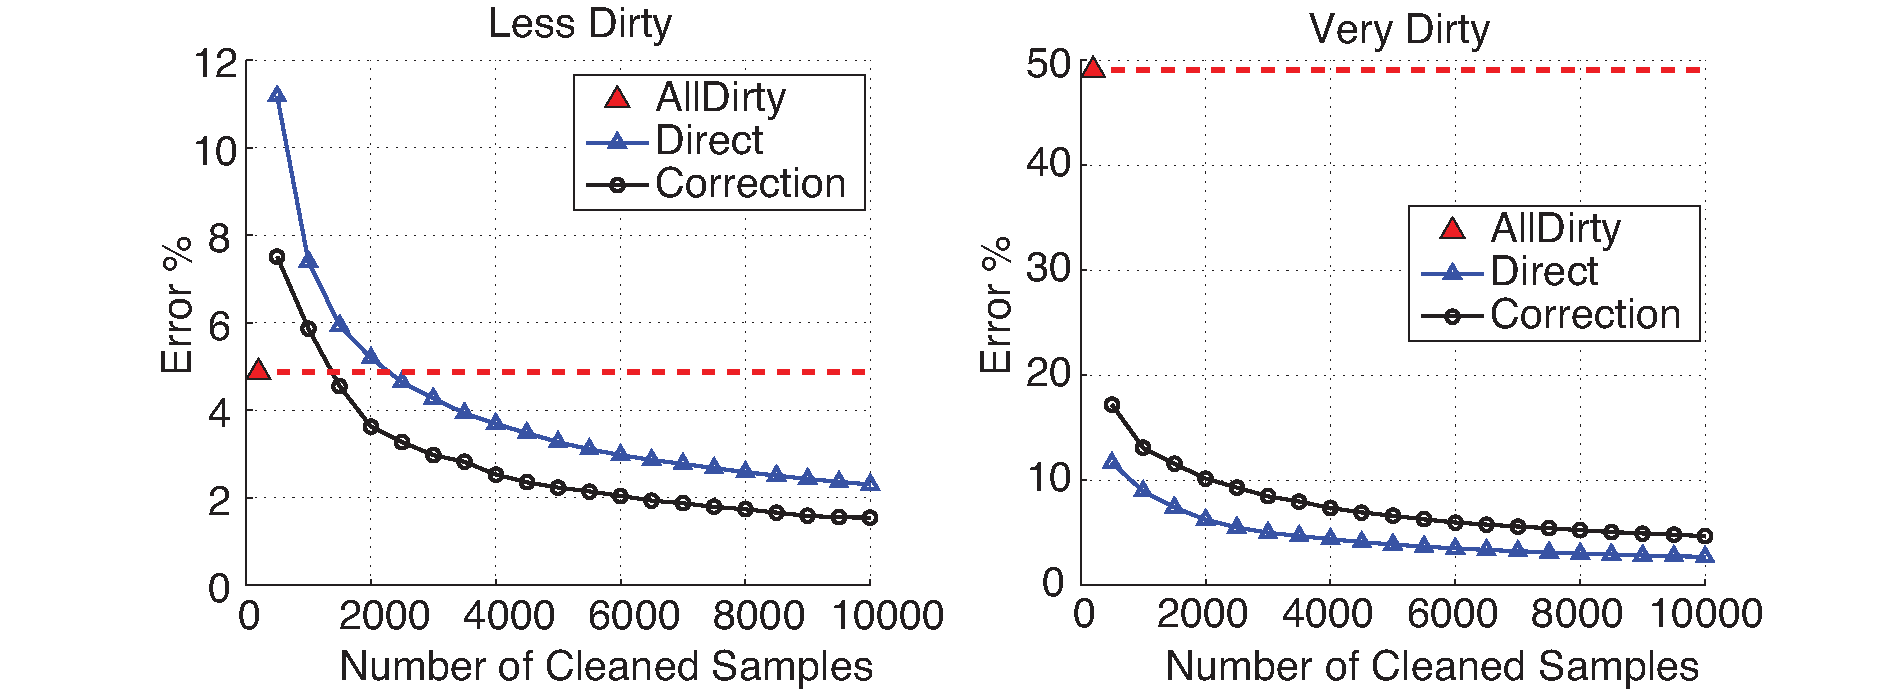
\includegraphics[width=.6\columnwidth]{figs/allerror-samplesize.pdf}
\caption{Comparison of the convergence of the methods on two TPC-H datasets of 6M tuples with simulated errors 50\% error and 5\% error. On the dataset with larger errors, the direct estimate gives a narrower confidence interval, and on the other the correction is more accurate. \label{fig:est2}}
\end{SCfigure}
\fi



